\chapter{User manual}\label{ch:user-guide}

\section{Overview}

This chapter shows a step-by-step guide on the usage of the tools developed for the users. Two guides are presented, one corresponding to each final product of the project:

\begin{itemize}
\item \textit{Web application guide:} Guide to the usage of the browser based client.

\item \textit{Mobile application guide:} Guide to the usage of the functions offered exclusively by the mobile application.
\end{itemize}

\section{Web application guide}

\subsection{Homepage}

The homepage is the first view the user finds when entering the web application. It presents a slider with the latest activity on the application shown in a map. In addition, it provides links to the mobile application, to the map, to the route uploading function and to a page explaining geolocated notes.

The appeareance of the homepage is shown on figure \ref{fig:homepage}.

\begin{figure}[ht]
  \centering
  \begin{subfigure}{.45\textwidth}
    \centering
    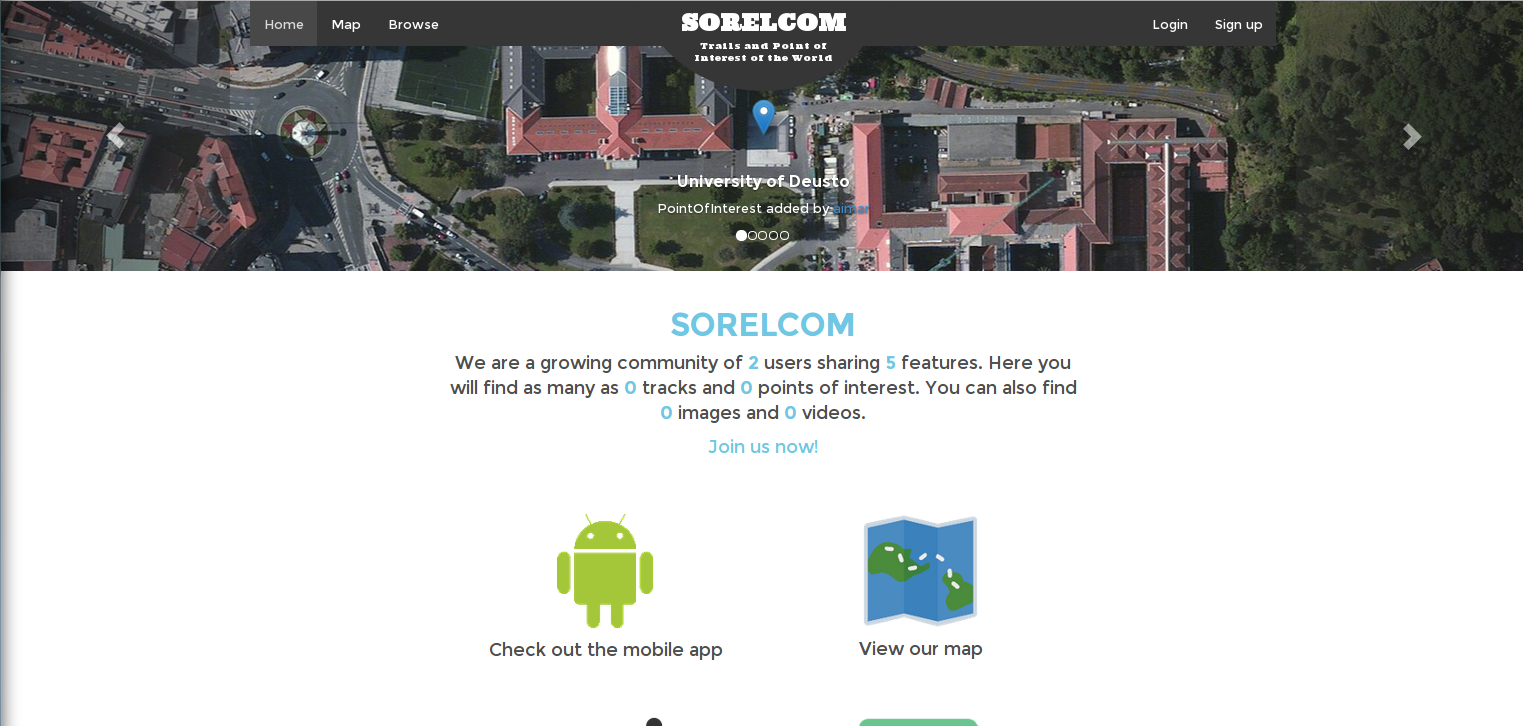
\includegraphics[width=.9\textwidth]{fig/homepage}
  \end{subfigure}
  \begin{subfigure}{.45\textwidth}
    \centering
    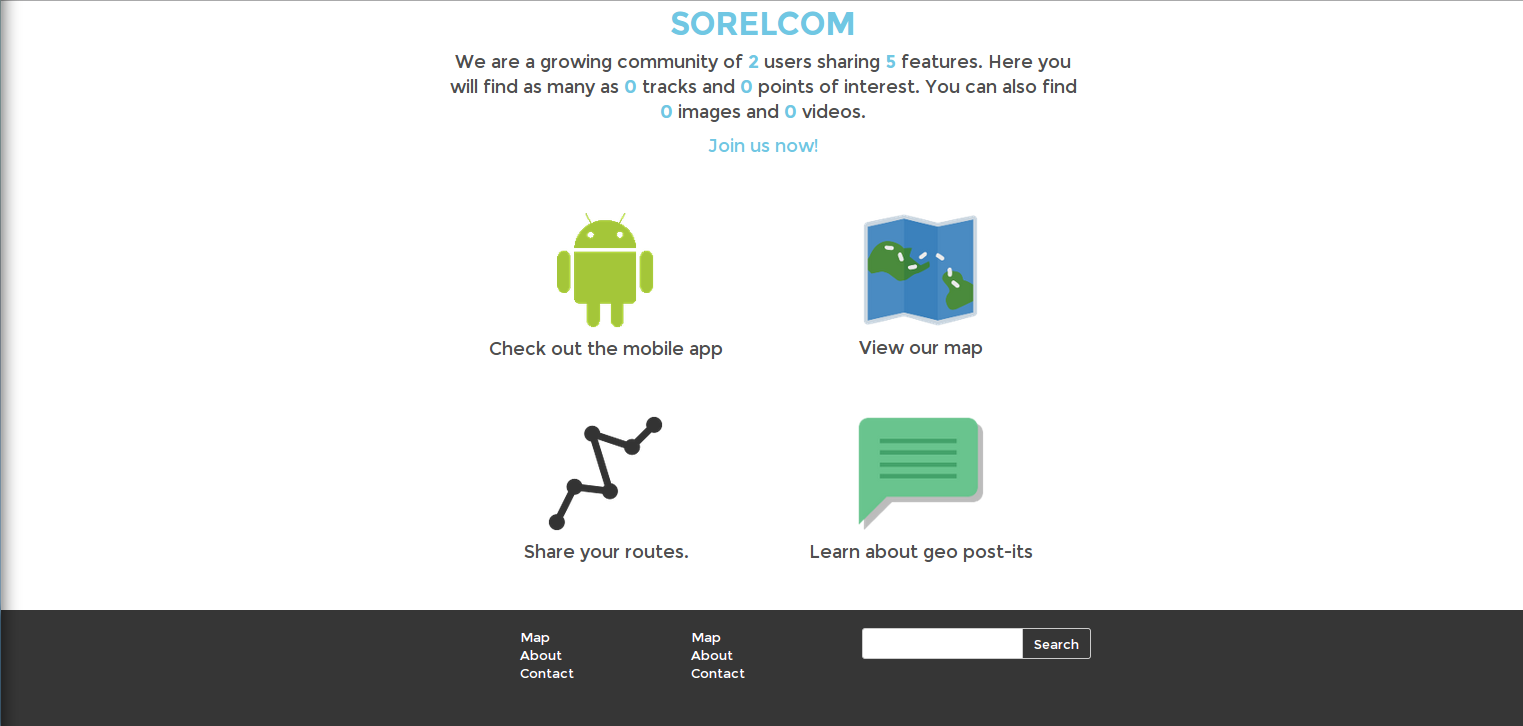
\includegraphics[width=.9\textwidth]{fig/homepage-bottom}
  \end{subfigure}  
  \caption{SORELCOM web application home page}
  \captionsetup{font={footnotesize,bf,it}}
  \label{fig:homepage}
\end{figure} 

\subsection{Navigation bar}

The navigation bar is a element that appears on most views on the web application. It provides links to the different sections of the web, such as the map editor and the search page. It also has a link to the sign up and login pages, which are changed for a link to the profile and a logout option when the user is logged in. The navbar can be found in figure \ref{fig:navbar}

\begin{figure}[ht]
  \centering
  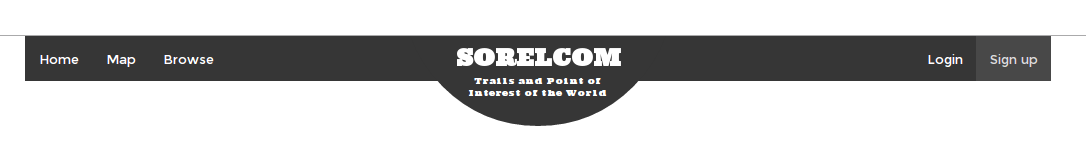
\includegraphics[width=.9\textwidth]{fig/navbar}
  \caption{SORELCOM web application navigation bar}
  \captionsetup{font={footnotesize,bf,it}}
  \label{fig:navbar}
\end{figure}

\subsection{World Map}

The world map is a view which takes the whole screen and shows a interactive map of the world. Through it, the features on the world can be explores, and the trail editor can be accessed.

The interface provided is based on two components, the map itself and a sidebar. This sidebar is open by default but it can be hidden using the button at the upper-right corner. Even when closed, a thing button will appear at one side of the application to allow the reopening of the sidebar.

The two states of the map, open sidebar and closed sidebar, are pictured in figure \ref{fig:map-view}.

\begin{figure}[ht]
  \centering
  \begin{subfigure}{.45\textwidth}
    \centering
    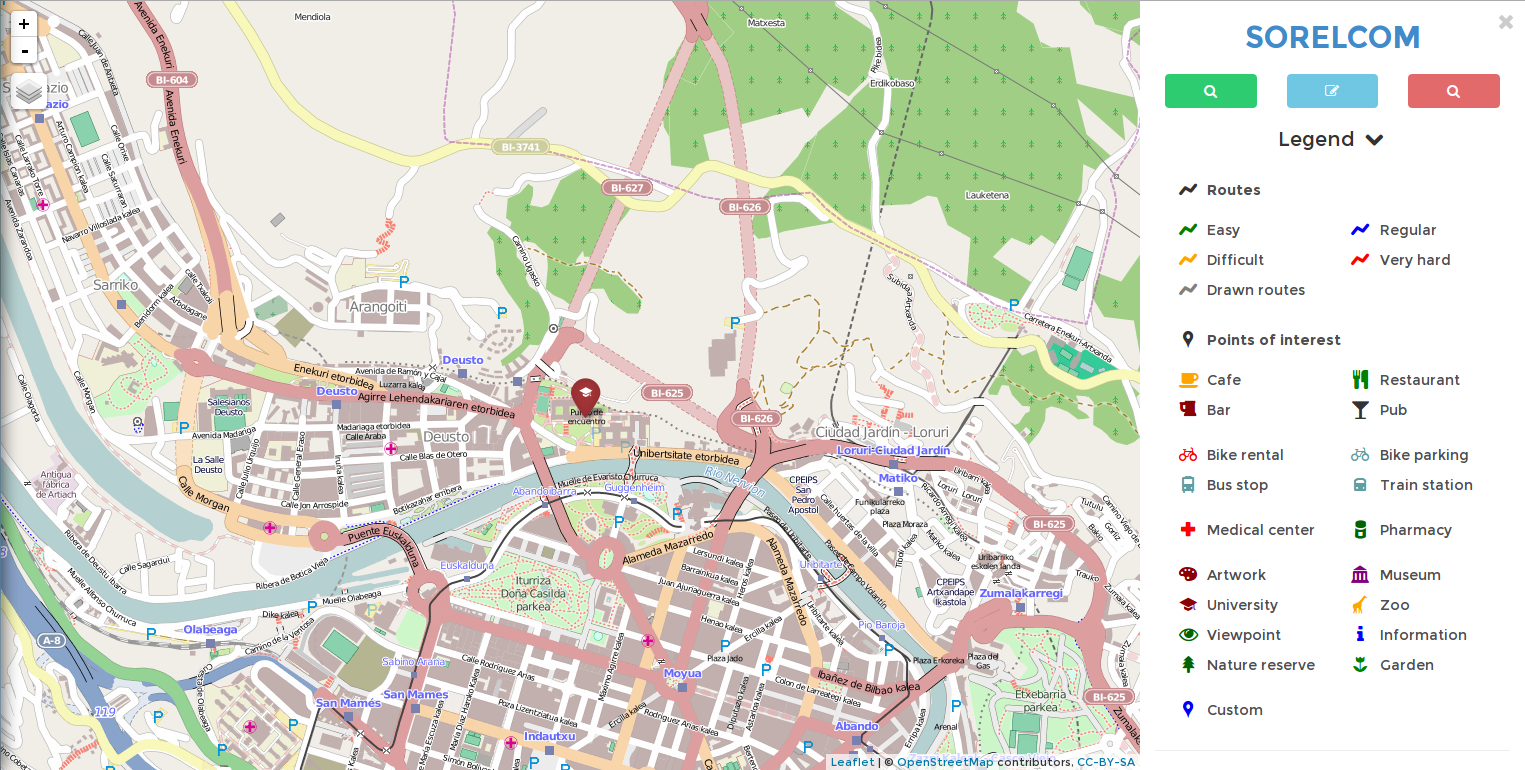
\includegraphics[width=.9\textwidth]{fig/map-explore-sidebar}
  \end{subfigure}
  \begin{subfigure}{.45\textwidth}
    \centering
    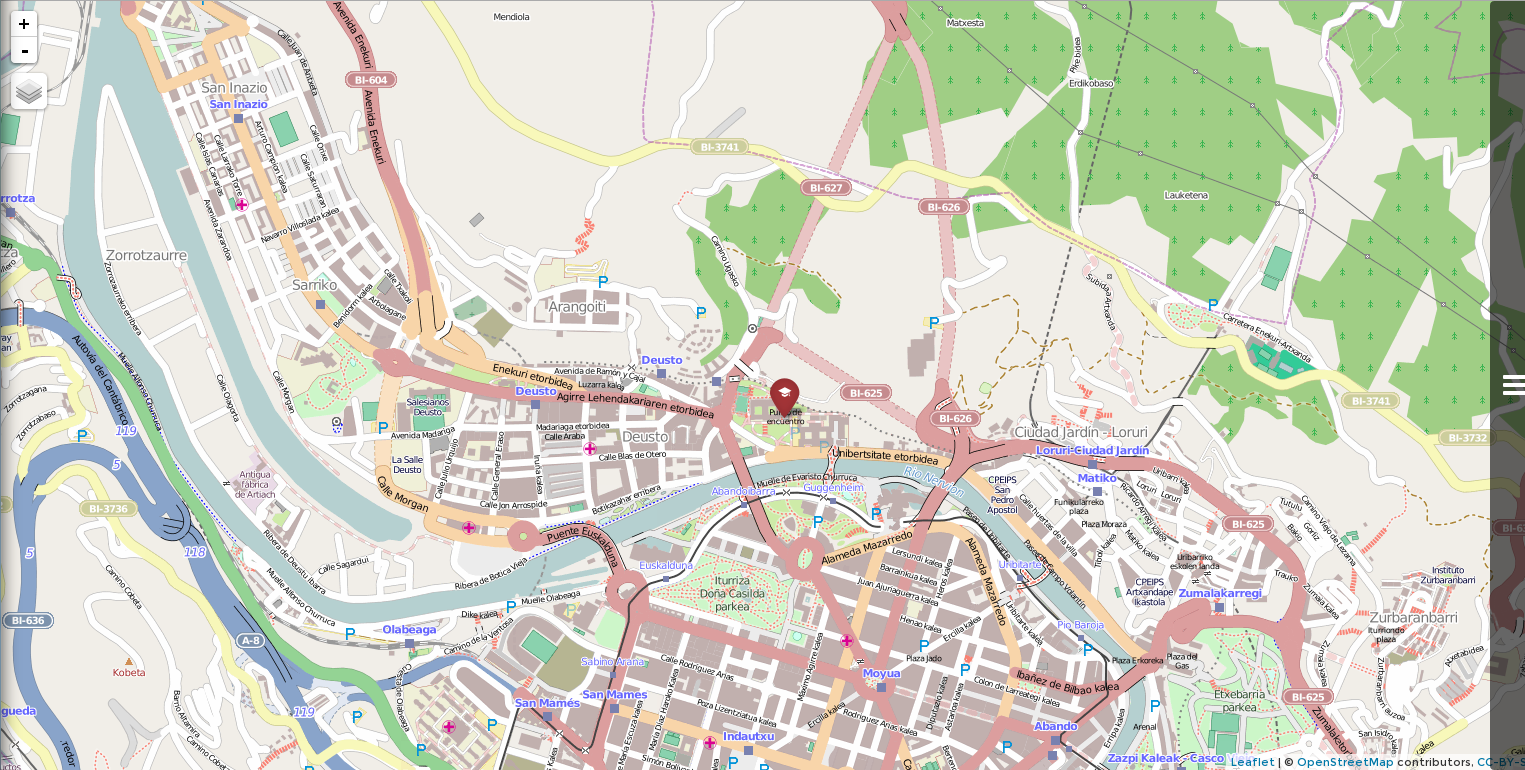
\includegraphics[width=.9\textwidth]{fig/map-explore-no-sidebar}
  \end{subfigure}  
  \caption{SORELCOM web application map view}
  \captionsetup{font={footnotesize,bf,it}}
  \label{fig:map-view}
\end{figure} 

The sidebar has its own navigation menu, composed by three small buttons. The first button offers the explorer sub-menu, the second button gives access to the editor functions and the third button has been left there to be expanded with a alternative explorer view on future iterations.

The basic editor view can be seen in figure \ref{fig:editor}

\begin{figure}[ht]
  \centering
  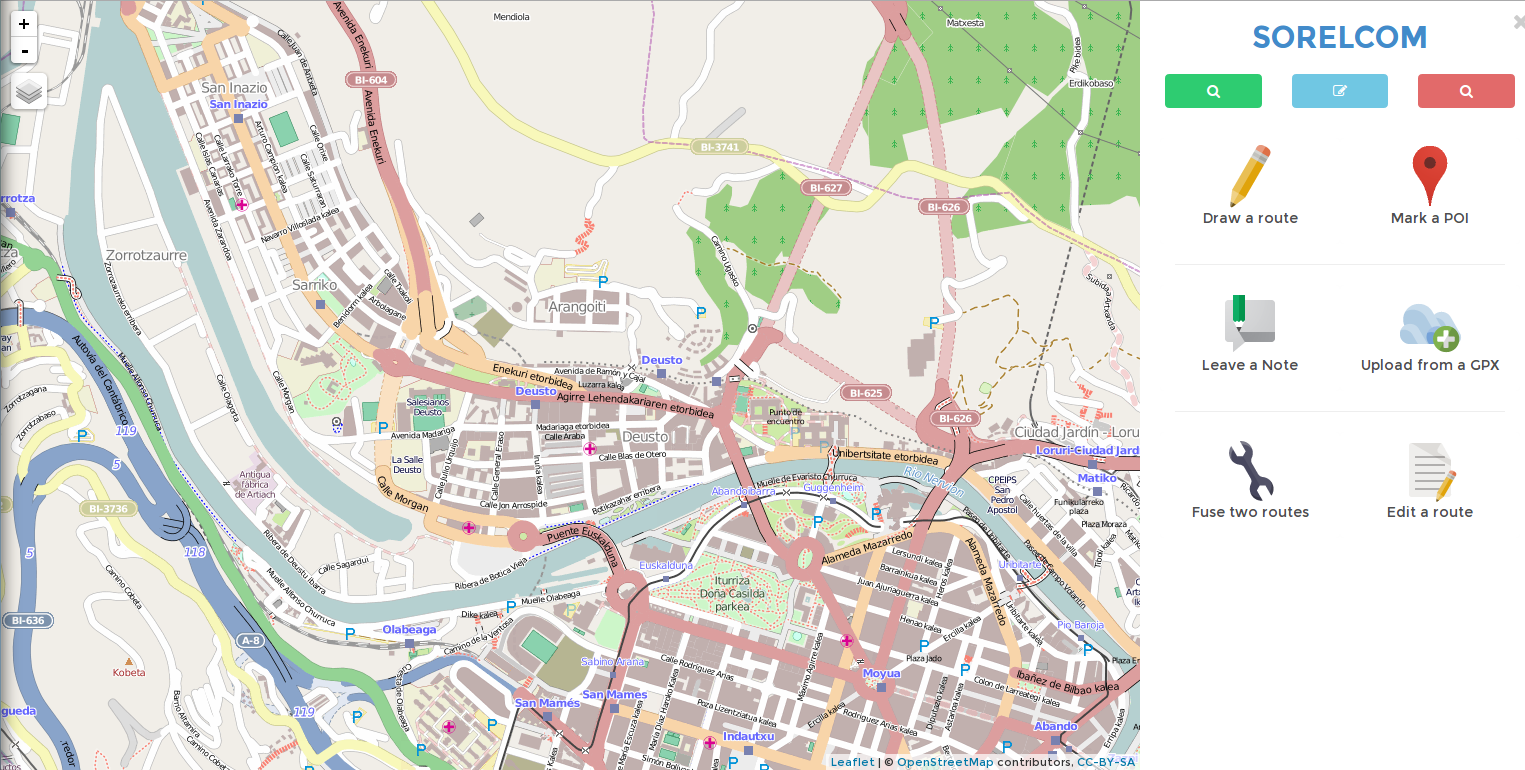
\includegraphics[width=.75\textwidth]{fig/map-editor}
  \caption{SORELCOM web application editor}
  \captionsetup{font={footnotesize,bf,it}}
  \label{fig:editor}
\end{figure}

\subsection{Editor}

When the editor is open, six buttons are presented on the sidebar. Each of these buttons gives access to one feature of the editor:

\subsubsection*{Route drawing}
When the button for drawing a route is clicked, the user is shown a tooltip on top of the map. This tooltip is used on the editor to give instructions on how to perform different actions. Once the user clicks on the map, the trail will be started there and a circle representing the 500 meter radius around will be shown. In order to add coordinates to the route, the user will have to click inside this circle, and the circle will move to represent the radius around the new coordinate.

Once the trail is finished, a button in the lower part of the map can be used to upload it. A cancel button is also provided to stop the creation of routes at any moment, and if the user leaves the editor view, this action will also be canceled and the map will be cleaned.

The interface for this is shown on figure \ref{fig:editor}.

\begin{figure}[ht]
  \centering
  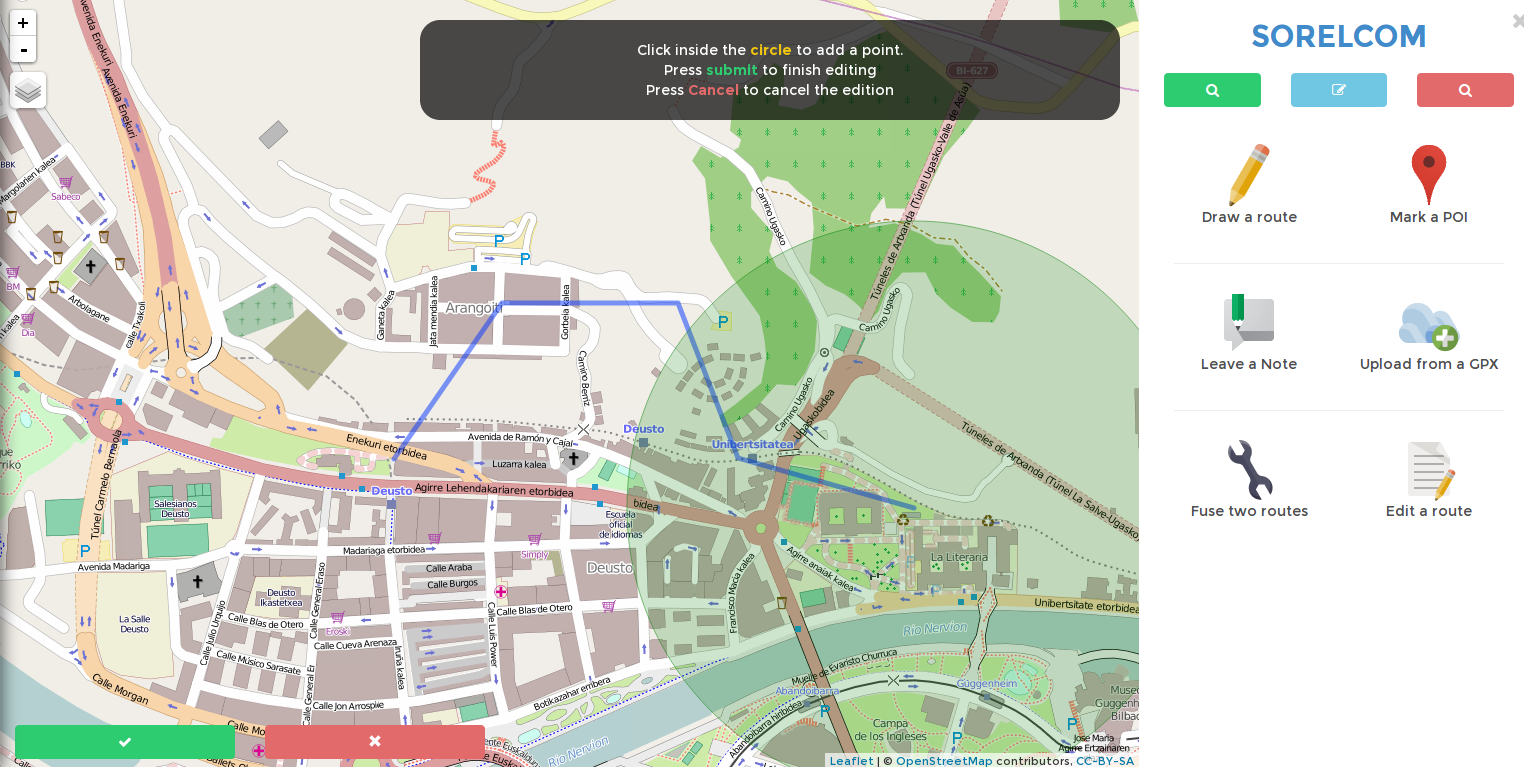
\includegraphics[width=.75\textwidth]{fig/draw-trail}
  \caption{SORELCOM web application trail drawing interface}
  \captionsetup{font={footnotesize,bf,it}}
  \label{fig:trail-draw}
\end{figure}


\subsubsection*{Point of interes and Geolocated note marking}

Marking a Point of Interest, or a Geolocated Note are done in the same manner. Once the button is clicked, the user only needs to click on the map and it will be prompted with a dialog with the form that needs to be filled in order to create the feature. This form requires very little information, however, it will vary depending on the type of feature created.

This same dialog is used when a GPX file is uploaded and when a trail is created in order to obtain the data needed to upload the information. This interface element can be found on figure \ref{fig:create}.

\begin{figure}[ht]
  \centering
  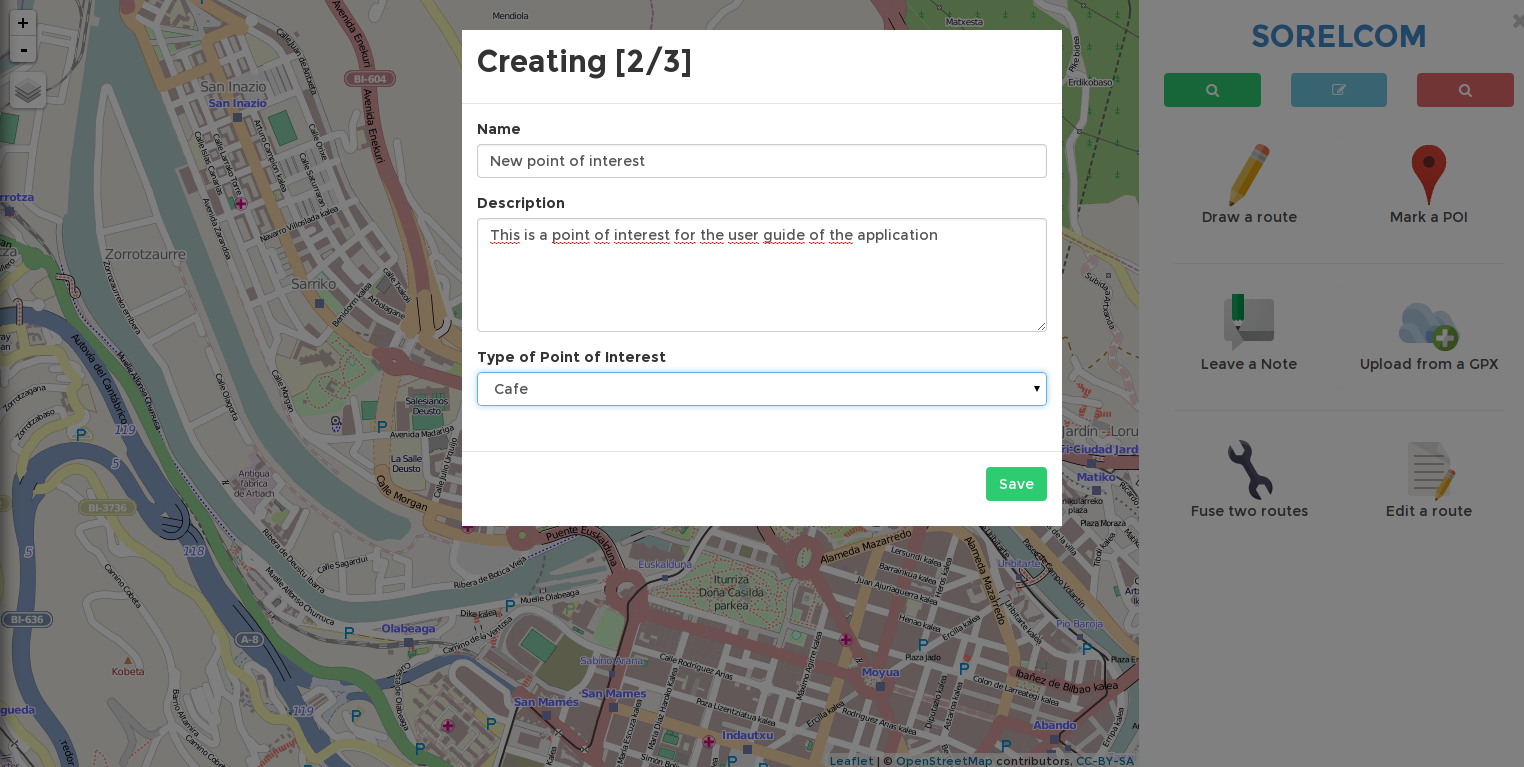
\includegraphics[width=.75\textwidth]{fig/mark-poi}
  \caption{SORELCOM web application feature creation dialog}
  \captionsetup{font={footnotesize,bf,it}}
  \label{fig:create}
\end{figure}

Once the data of a feature has been created and saved, the dialog shown in figure \ref{fig:upload} will be prompted, allowing the user to upload media files to the feature. This dialog reads one or multiple files and shows a preview of them to the user. This preview can be clicked in order to prevent the uploading of a concrete file.

Once all the files are added, the button in the bottom of the dialog can be used to start the upload. Any file successfully saved will be removed from the preview list, however, if there is errors in any of them a message will appear on the screen.

\begin{figure}[ht]
  \centering
  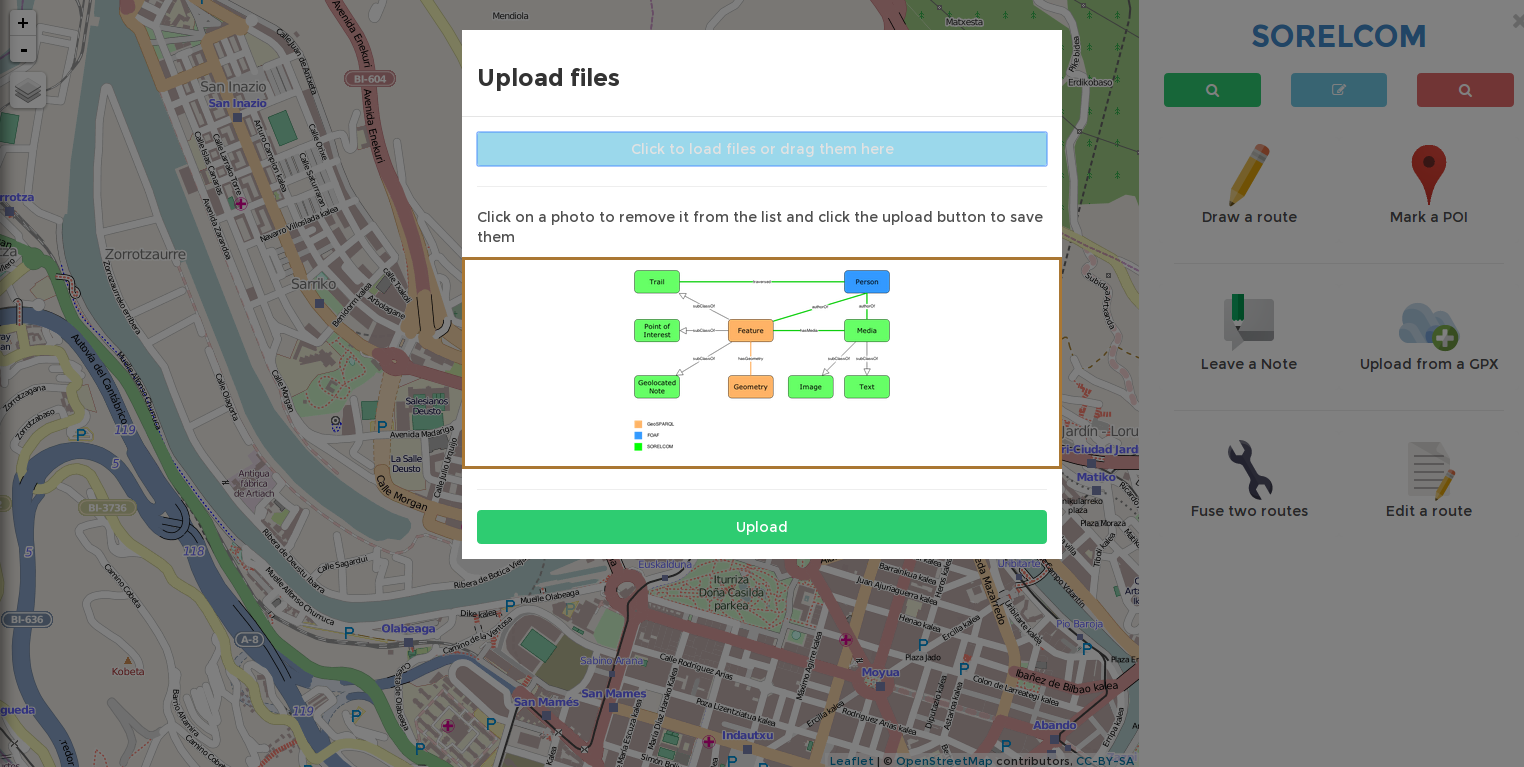
\includegraphics[width=.75\textwidth]{fig/upload-file}
  \caption{SORELCOM web application media upload dialog}
  \captionsetup{font={footnotesize,bf,it}}
  \label{fig:upload}
\end{figure}

\subsubsection*{GPX import}

When the button for uploading a GPX file is clicked, a dialog used to load this kind of files is opened. This dialog provides a button which is used to browse a local file. Once this file is selected, the application will read the file and parse all the features in it. The features will be presented on small maps, and the user will have to select one in order to proceed, as shown in figure \ref{fig:gpx-import}. Once it is done, the process of saving it will be the same as when marking a point of interest.

\begin{figure}[ht]
  \centering
  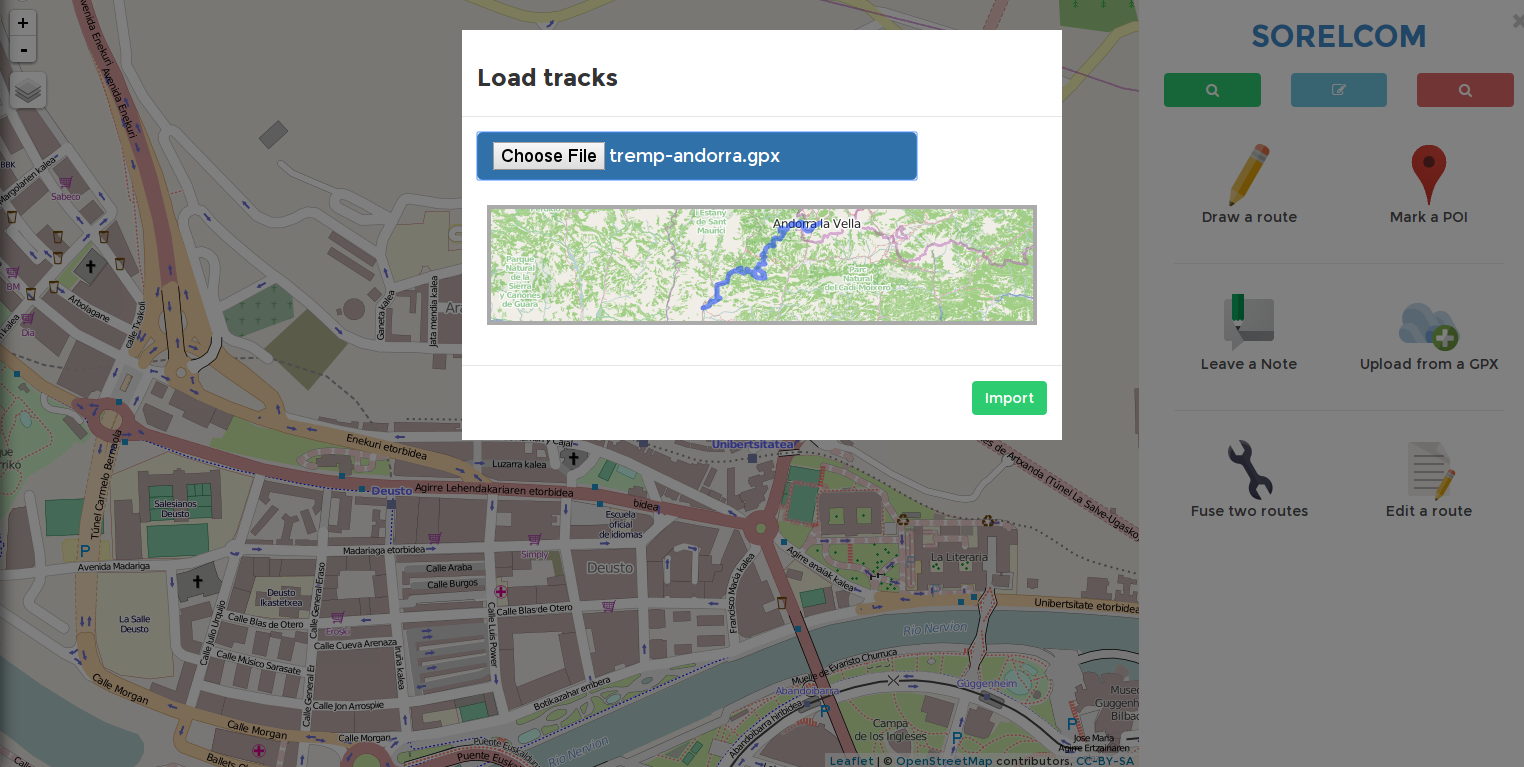
\includegraphics[width=.75\textwidth]{fig/trail-import-select}
  \caption{SORELCOM web application GPX loading dialog}
  \captionsetup{font={footnotesize,bf,it}}
  \label{fig:gpx-import}
\end{figure}

\subsubsection*{Trail editing}

When the option of trail editing is chosen, two options are given, using a trail that already exists in the system or importing a GPX file, as shown in figure \ref{fig:options}.

\begin{figure}[ht]
  \centering
  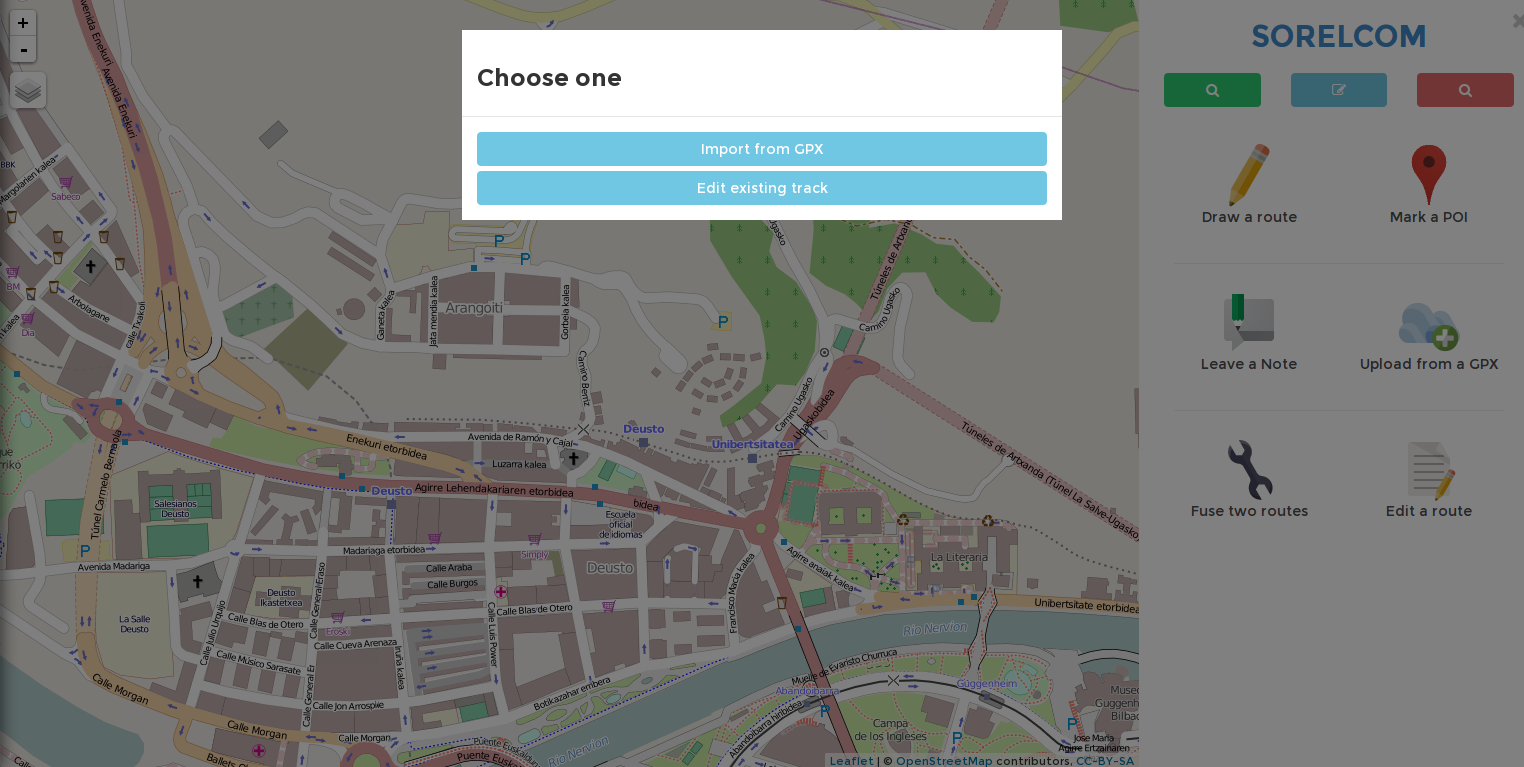
\includegraphics[width=.75\textwidth]{fig/trail-import}
  \caption{SORELCOM web application dialog to chose source of a trail}
  \captionsetup{font={footnotesize,bf,it}}
  \label{fig:options}
\end{figure}

If the option of downloading a trail from the server is chosen, another modal will appear listing the trails available. If the option of importing from a GPX file is chosen, then the same modal used for GPX loading will appear. Once a trail is chosen, it will be shown on the map, with the addition of a number of markers to edit the route.

By dragging this markers, the coordinates on the route will me moved. Dragging a marker in the middle of a line will create a new coordinate between the points of that segment. Right clicking on a marker will delete a coordinate. Figure \ref{fig:trail-edit} shows a trail in the editor. It has been deformed to show how the coordinates can be moved around.

\begin{figure}[ht]
  \centering
  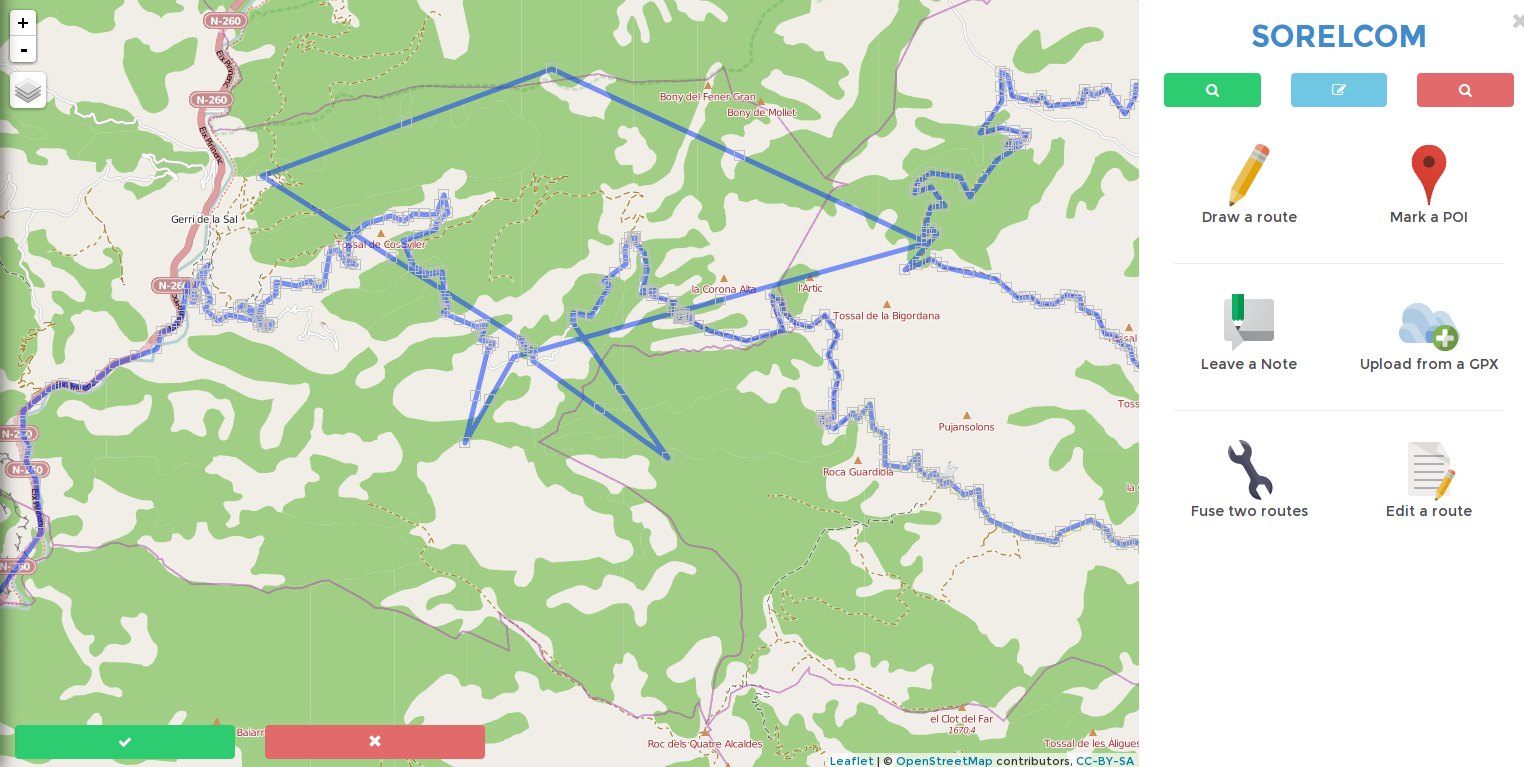
\includegraphics[width=.75\textwidth]{fig/trail-edit}
  \caption{SORELCOM web application interface for trail edition.}
  \captionsetup{font={footnotesize,bf,it}}
  \label{fig:trail-edit}
\end{figure}

Once the trail is edited, the user can click the green button at the bottom of the map to save the changes. If the trail already exists in the system it will be saved, if it does not, the same process followed after draw creation will start.

\subsubsection*{Route fusion}

Unfortunately, due to time constraints, it has been impossible to implement the route fusing functionality on the current date. When it is implemented, it will follow a similar procedure to that of editing a trail. 

Two dialogs will appear, each of them used to choose one route. Once both routes are chosen, they will be joined from the start of one of them to the end of the other, and shown in a map as editable trail.

\subsection{Explorer}

When the explorer is active, the sidebar shows a legend. This legend identifies the icon shown for each kind of point of interest, and the colors for each route depending on the difficulty score they have.

When the application is on the explorer view, the map will contain the points of interest and routes which appear on the current viewport. When one of these elements is clicked, a pop up will be shown with basic information about the feature and a link to the detailed view. An example of this is depicted in figure \ref{fig:explorer}.

\begin{figure}[ht]
  \centering
  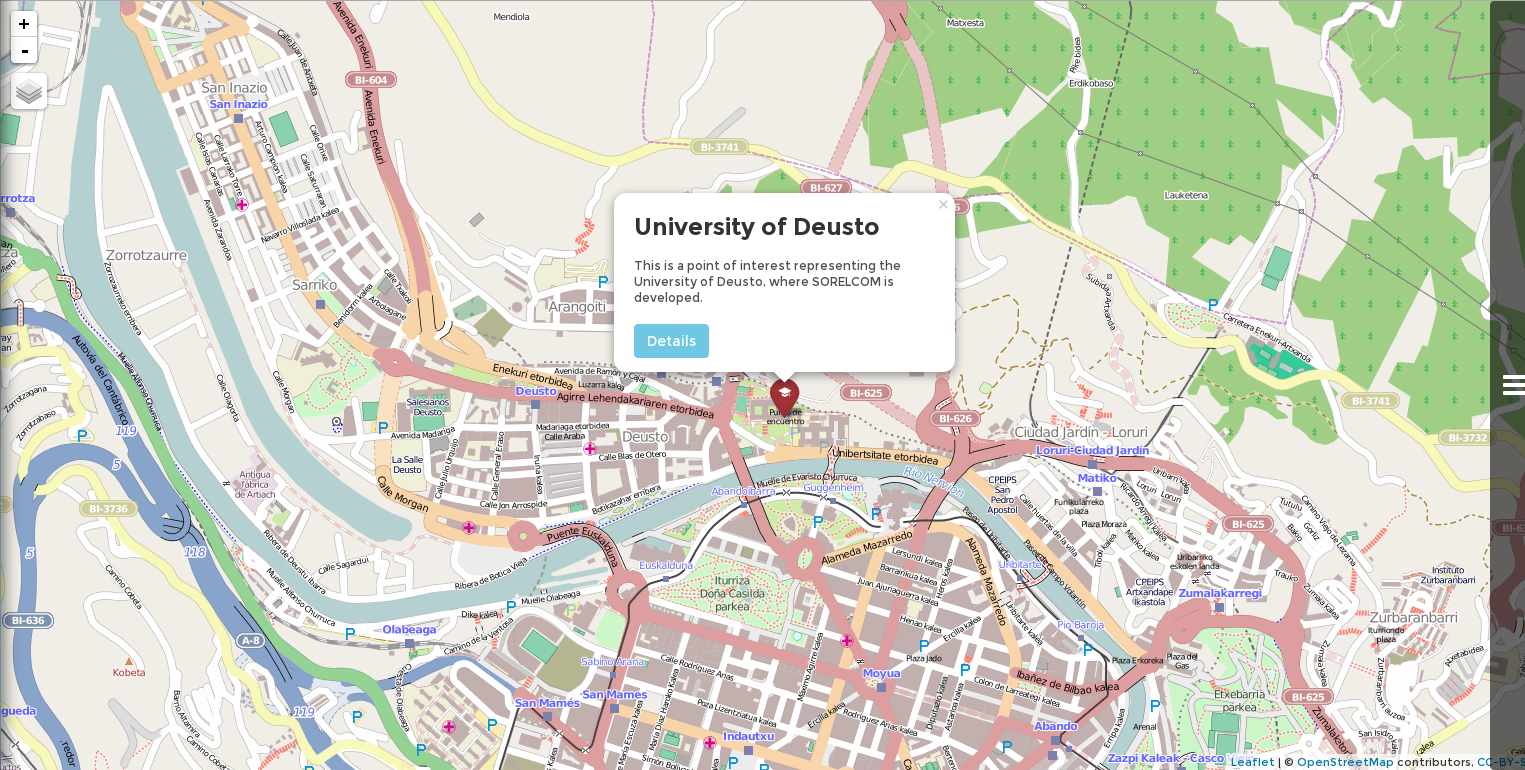
\includegraphics[width=.75\textwidth]{fig/map-explore-link}
  \caption{SORELCOM web application world map explorer interface}
  \captionsetup{font={footnotesize,bf,it}}
  \label{fig:explorer}
\end{figure}

\subsection{Search page}

The search page allows the user to make text based search over the features and users of the application. It can be accessed the same way as the map, through the navigation bar. This interface provides a simple box to enter a text to search and shows a list of results once the search is done. It is possible to access to the search page by using the input box on the footer of most pages of the application.

By clicking on one of the items of the list, the application will switch to a detailed view for it. A search example is shown on figure \ref{fig:search}.

\begin{figure}[ht]
  \centering
  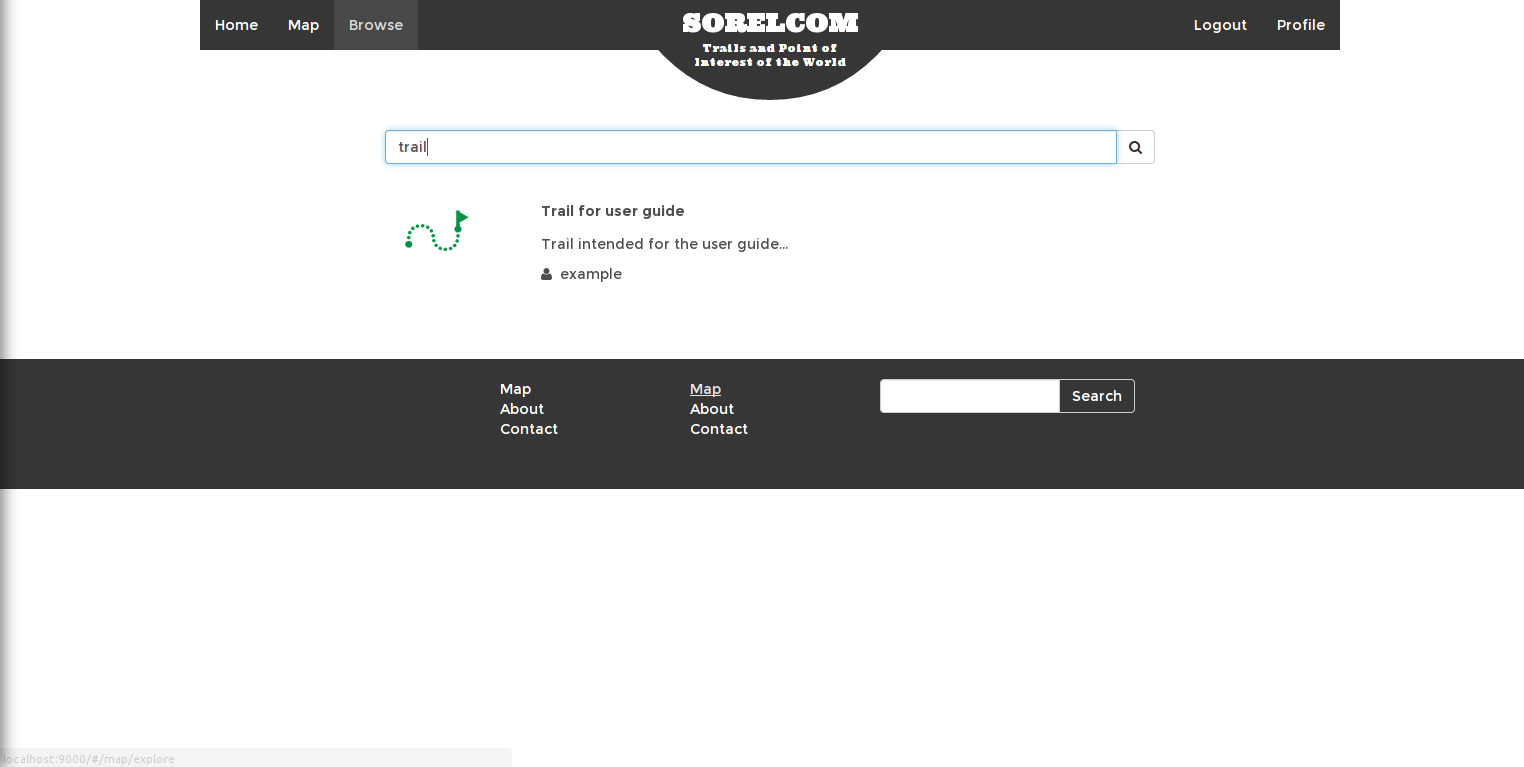
\includegraphics[width=.75\textwidth]{fig/search}
  \caption{SORELCOM web application search page}
  \captionsetup{font={footnotesize,bf,it}}
  \label{fig:search}
\end{figure}

\subsection{Feature view}

The feature view can be accessed through the items in the search page or by clicking on the link on the map explorer pop up boxes. This view shows a small map centered on the feature and information about the feature. This information includes description, difficulty and spatial features.

In addition, the images that depict the feature will be shown (if there are any) and the reviews of the user on the application will be listed. It is also possible to post a review on the application though the text box before the comments, however, the numerical rating has not yet been implemented on the interface.

Figure \ref{fig:feature-view} shows a detailed view of a point of view previously marker on the map editor view.

\begin{figure}[ht]
  \centering
  \begin{subfigure}{.45\textwidth}
    \centering
    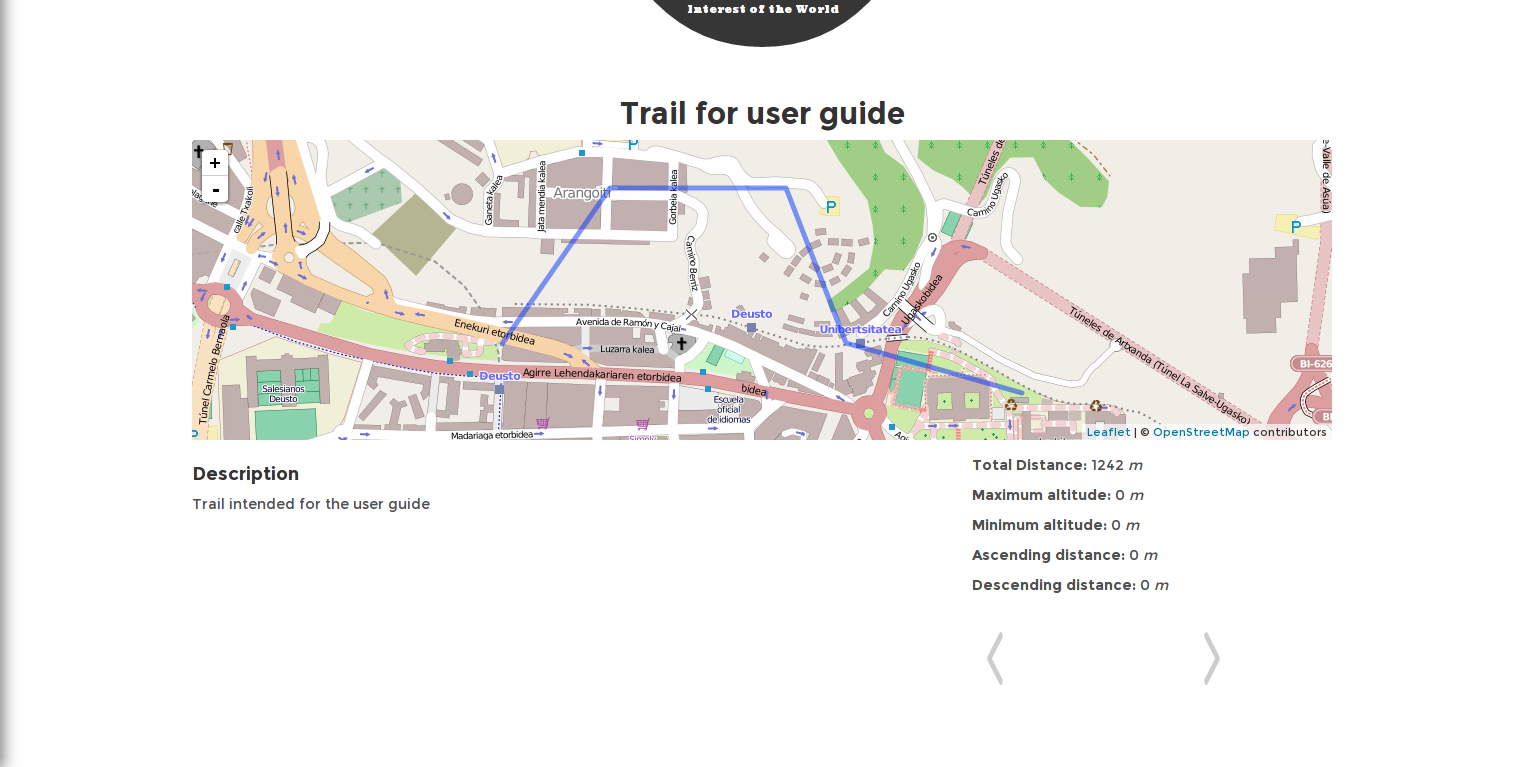
\includegraphics[width=.9\textwidth]{fig/trail-view}
  \end{subfigure}
  \begin{subfigure}{.45\textwidth}
    \centering
    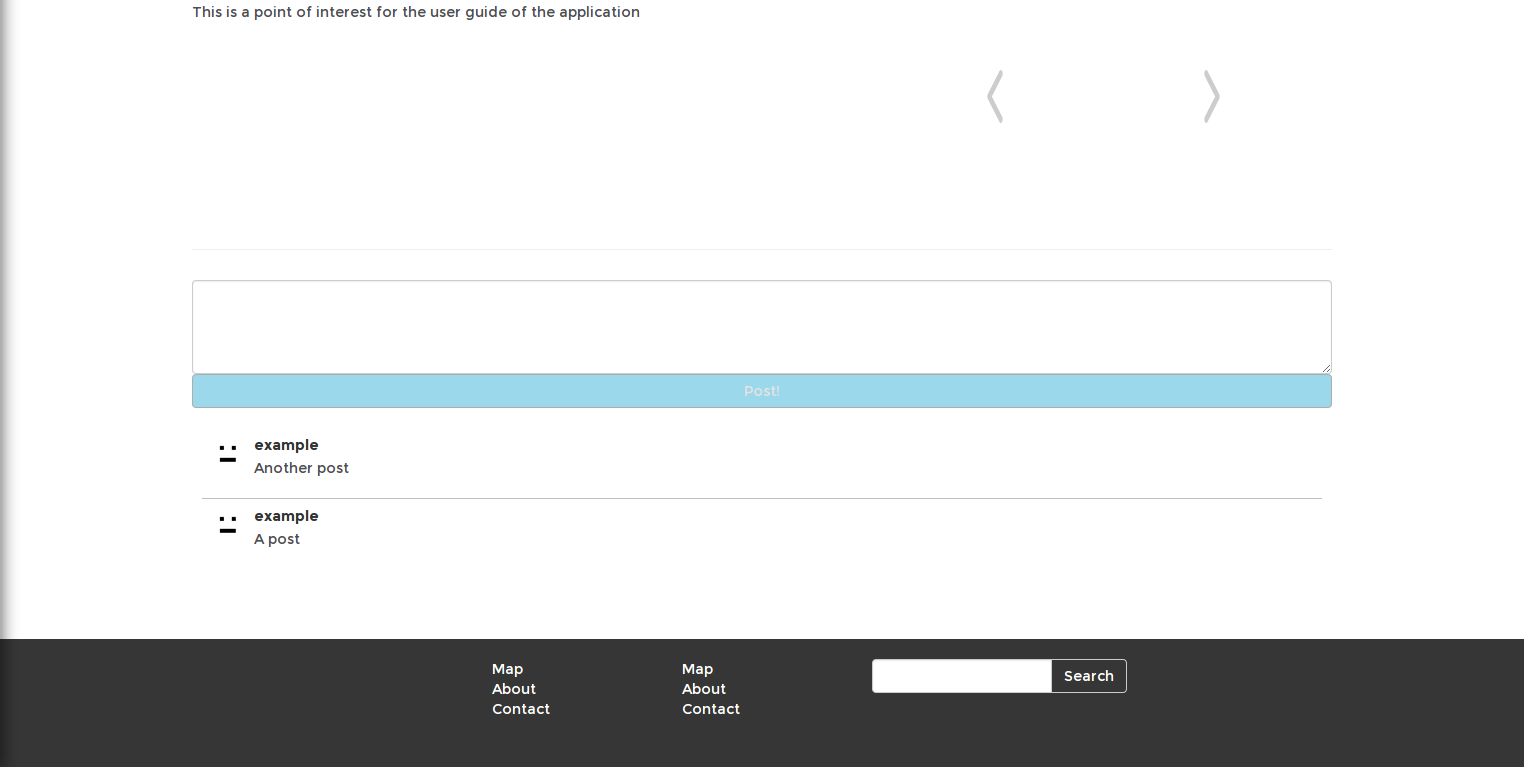
\includegraphics[width=.9\textwidth]{fig/post-view}
  \end{subfigure}  
  \caption{SORELCOM web application feature view showing a drawn trail}
  \captionsetup{font={footnotesize,bf,it}}
  \label{fig:feature-view}
\end{figure} 

\subsection{User view}

The user view is the analogous to the feature view regarding information of the users. This view shows the profile picture, the email and the nickname of the user. In addition, a small navigation menu is provided that allows to choose between viewing the trails, points of interest, buddies and followers of the user.

If someone is logged in the application and the user being viewed is different from the one signed in the system, two buttons are shown, to follow and add a user as a buddy. This interface is shown in figure \ref{fig:user-view}.

\begin{figure}[ht]
  \centering
  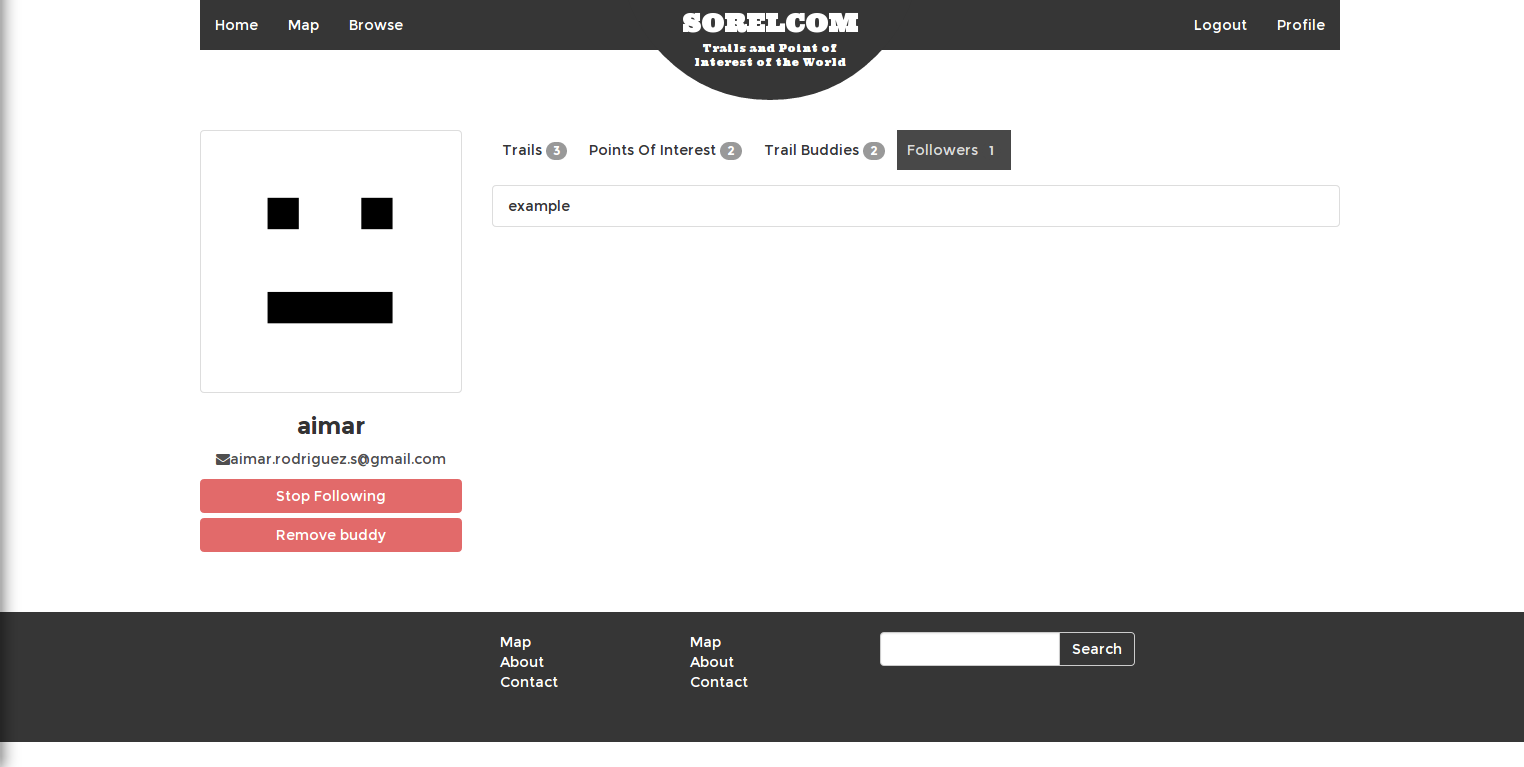
\includegraphics[width=.75\textwidth]{fig/user}
  \caption{SORELCOM web application user view}
  \captionsetup{font={footnotesize,bf,it}}
  \label{fig:user-view}
\end{figure}

\subsection{Registration}

Many of the functions on the web application require registration of the user in the platform. This is done through the sign up page, accessible from the homepage and the navigation bar. The sign up page shows a form requiring user name, email and password to create the user, as shown in figure \ref{fig:sign-up}.

\begin{figure}[ht]
  \centering
  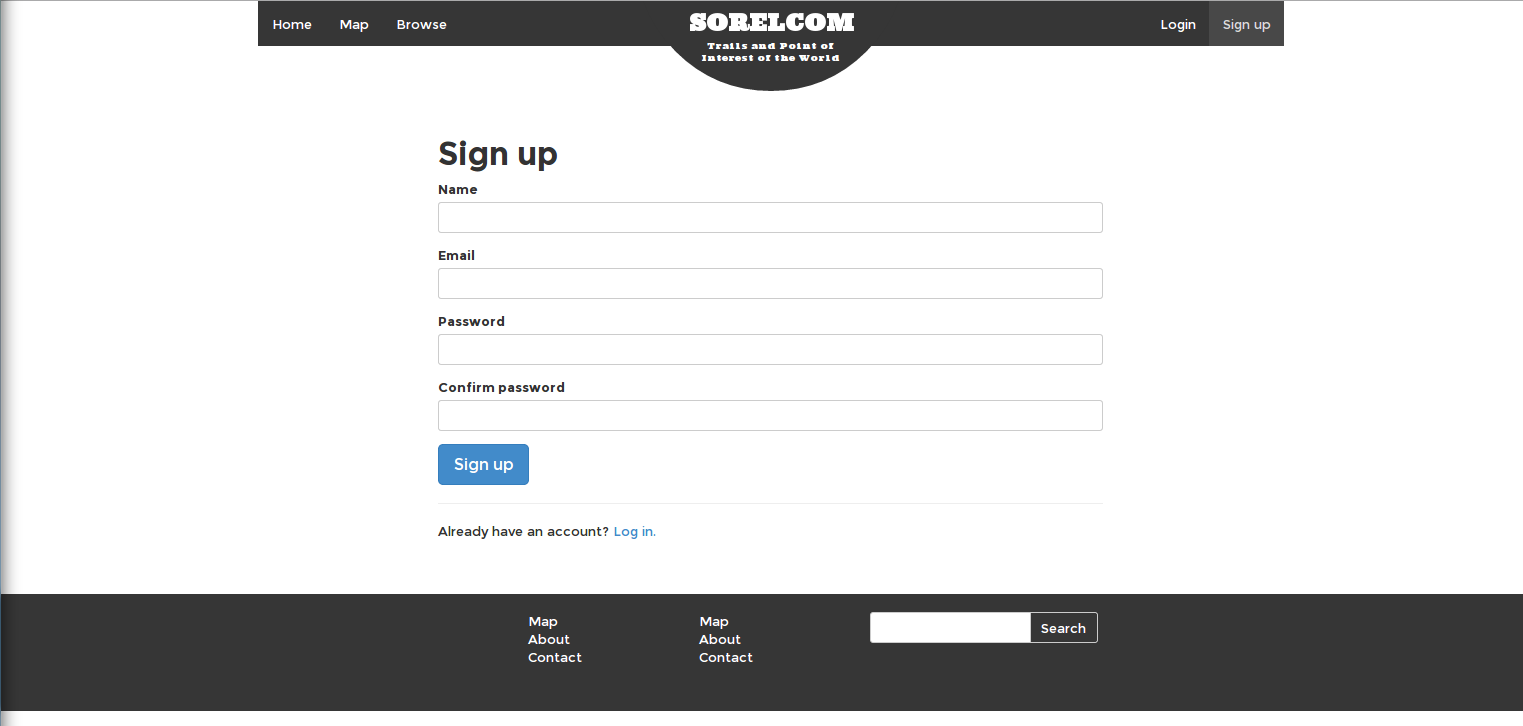
\includegraphics[width=.75\textwidth]{fig/sign-up}
  \caption{SORELCOM web application sign up form}
  \captionsetup{font={footnotesize,bf,it}}
  \label{fig:sign-up}
\end{figure}

Once a person is registered in the application it will automatically log in the application. 

\subsection{Sign in}

In order to sign in, a dialog is used. This is done to provide the login functionality at any point required without disrupting the flow of actions of the user. In addition, this dialog can be accessed from the navigation bar.

The interface for signing in is show in figure \ref{fig:login}. The user name or email and a password are required. Once the login is successful the modal closes, and if there was some pending operation it is executed.

\begin{figure}[ht]
  \centering
  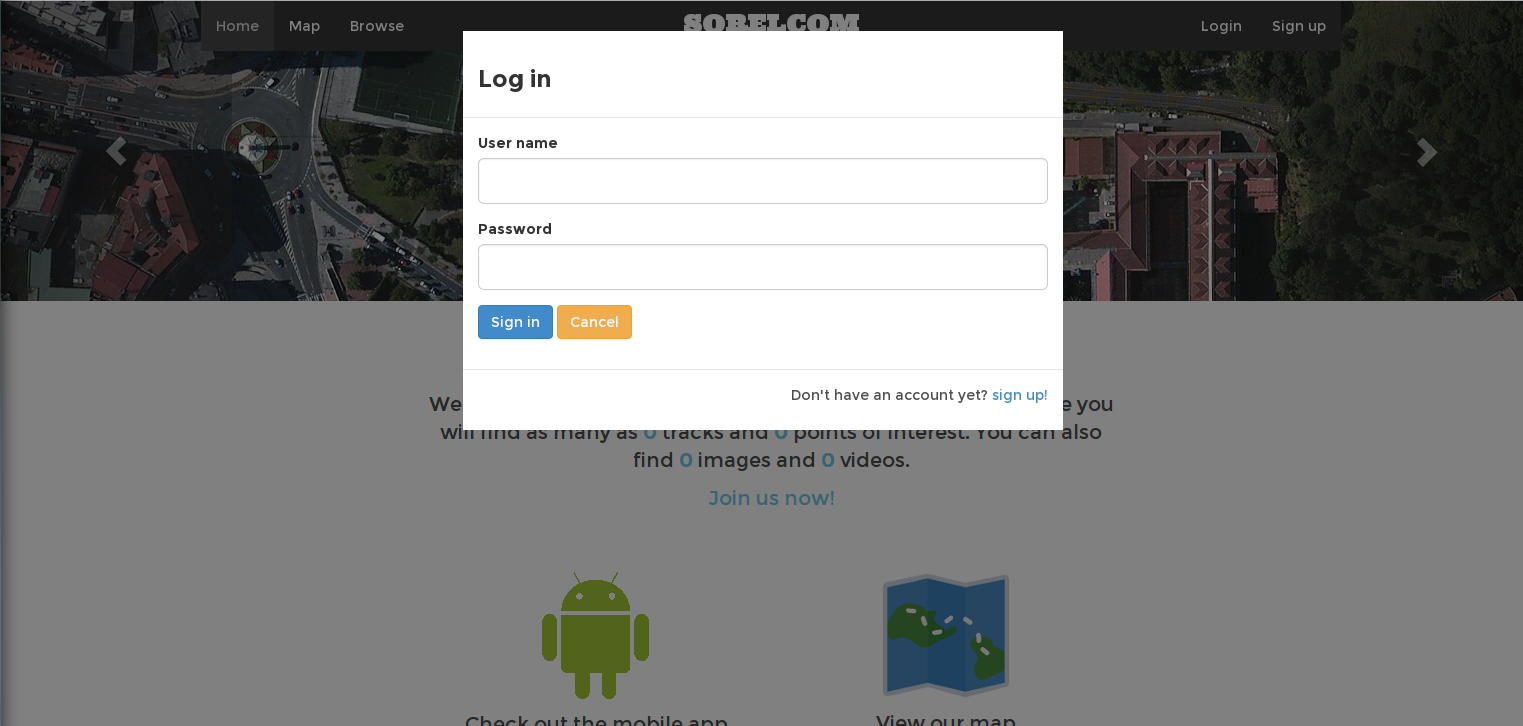
\includegraphics[width=.75\textwidth]{fig/login}
  \caption{SORELCOM web application login dialog}
  \captionsetup{font={footnotesize,bf,it}}
  \label{fig:login}
\end{figure}

\subsection{User profile}

The user profile page is used to configure the personal profile of the logged user. This function is only used when a person is signed in the application. It offers a overview of the same information the user can see in the user view page, in addition to a form to update the information about a user.

Recommendations are also shown in a list on this page, which are recalculated every time the user profile is opened. The profile page is shown on figure \ref{fig:profile}.

\begin{figure}[ht]
  \centering
  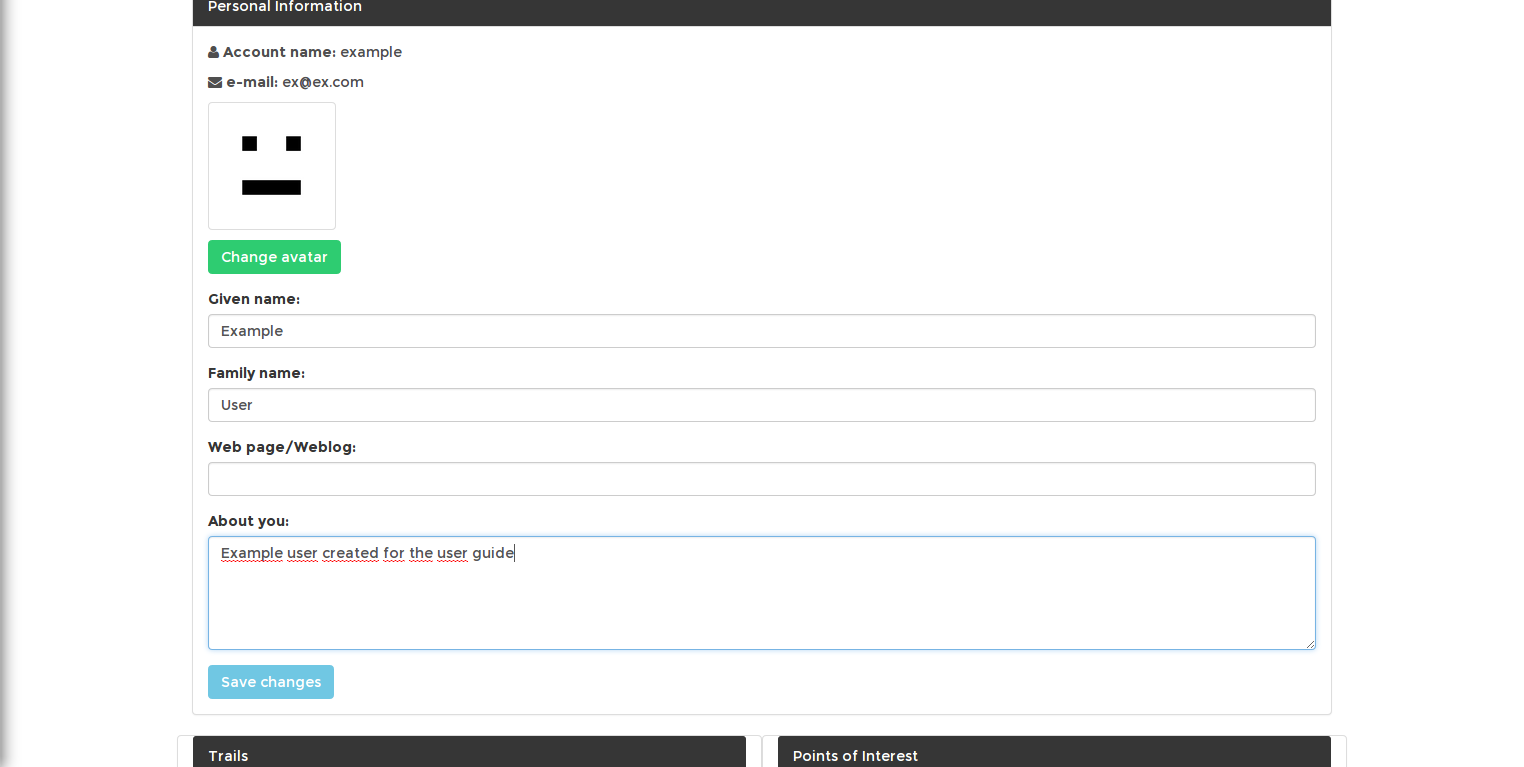
\includegraphics[width=.75\textwidth]{fig/profile}
  \caption{SORELCOM web application user profile}
  \captionsetup{font={footnotesize,bf,it}}
  \label{fig:profile}
\end{figure}

\subsection{Mobile web}

The web offers the same functions when accessed through the mobile interface, however, due to the narrow screens, the views have been restructured. The most prominent example of this is the world map.

The sidebar of the world map will take the full screen when on a mobile device, so it will have to be hidden in order to actually see the map. However, it is still possible to user all the functions even with only touch buttons. This example is shown in figure \ref{fig:mobile-web}

\begin{figure}[ht]
  \centering
  \begin{subfigure}{.45\textwidth}
    \centering
    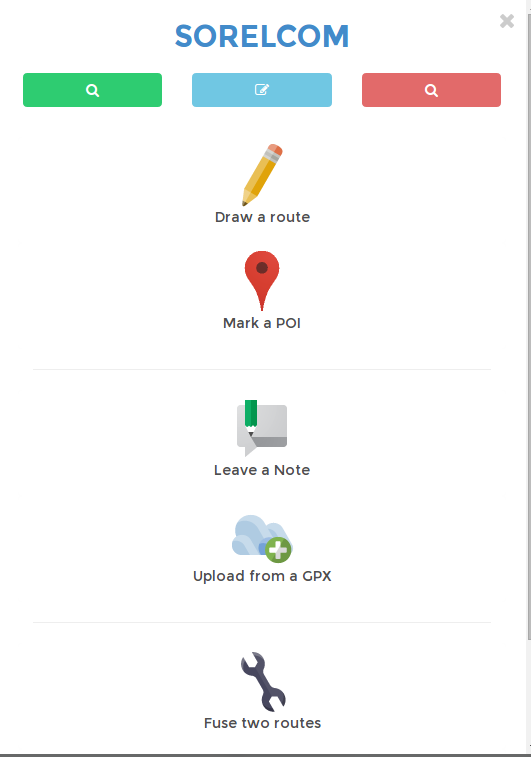
\includegraphics[width=.8\textwidth]{fig/responsive1}
  \end{subfigure}
  \begin{subfigure}{.45\textwidth}
    \centering
    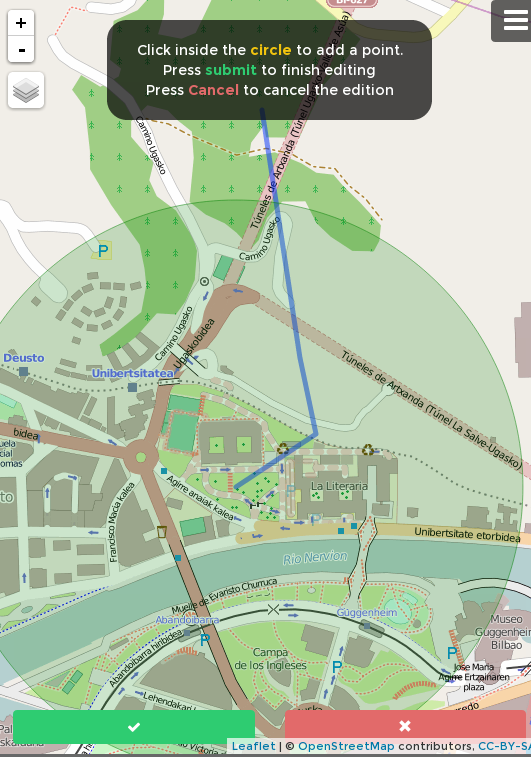
\includegraphics[width=.8\textwidth]{fig/responsive2}
  \end{subfigure}  
  \caption{SORELCOM web application on a mobile device}
  \captionsetup{font={footnotesize,bf,it}}
  \label{fig:mobile-web}
\end{figure} 